% Compilar con XeLaTeX o LuaLaTeX (en Overleaf: Menu -> Compiler -> XeLaTeX)
\documentclass[11pt, a4paper]{article}

\usepackage[a4paper, margin=2.3cm, top=2.6cm, bottom=2.6cm]{geometry}
\usepackage{fontspec}
\usepackage[english, spanish, provide=*]{babel}
\IfFontExistsTF{Noto Sans}{\babelfont{rm}{Noto Sans}}{}

\usepackage{amsmath,amssymb}
\usepackage{xcolor}
\setlength{\headheight}{14pt}
\usepackage{booktabs}
\usepackage{graphicx}
\usepackage{array}
\usepackage{caption}
\captionsetup{font=small, labelfont=bf}
\usepackage{fancyhdr}
\usepackage{hyperref}
\hypersetup{colorlinks=true, linkcolor=blue!50!black, citecolor=blue!50!black, urlcolor=blue!50!black}
\graphicspath{{../figs/}{figs/}}

\pagestyle{fancy}
\fancyhf{}
\lhead{Asignación Mecánica Clásica: Troyanos de Júpiter}
\rhead{18/11/2026}
\lfoot{Ríos, Sarmiento}
\cfoot{Universidad Industrial de Santander}
\rfoot{\thepage}
\renewcommand{\headrulewidth}{0.4pt}
\renewcommand{\footrulewidth}{0.4pt}
\fancypagestyle{plain}{\fancyhf{}
  \lhead{Asignación Mecánica Clásica: Troyanos de Júpiter}\rhead{18/11/2026}
  \lfoot{Ríos, Sarmiento}\cfoot{Universidad Industrial de Santander}\rfoot{\thepage}
  \renewcommand{\headrulewidth}{0.4pt}\renewcommand{\footrulewidth}{0.4pt}}

\title{\vspace{-1.2cm}¿Hasta dónde sirve el análisis lineal?\\[2pt] \large Los troyanos de Júpiter frente a la teoría de pequeñas oscilaciones}
\author{Paola Andrea Ríos Campos \quad (Código 2240684) \\ Juan Diego Sarmiento Villarreal \quad (Código 2240676)\\[2pt]
\small Escuela de Física, Universidad Industrial de Santander, Bucaramanga, Colombia\\ \small Mecánica Clásica · Reto III.1}
\date{18 de noviembre de 2026}

\newcommand{\Tlin}{T_{\rm lin}}
\begin{document}
\maketitle
\thispagestyle{plain}


\begin{abstract}
\noindent Los asteroides troyanos comparten la órbita de Júpiter y libran alrededor de los puntos de Lagrange $L_4$ y $L_5$. La teoría clásica de pequeñas oscilaciones en el problema restringido circular de tres cuerpos (PR3C) predice que esta libración es armónica, con un período que depende solo de la razón de masas $\mu$: $\Tlin = 147{,}4$ años para el sistema Sol--Júpiter. Pero los troyanos reales no están infinitesimalmente cerca del equilibrio. Este trabajo cuantifica \emph{hasta qué amplitud} la descripción lineal sigue siendo confiable y \emph{qué fracción} de los troyanos conocidos cae dentro de ese rango.

Derivamos las ecuaciones de movimiento en el marco rotante con el formalismo lagrangiano, la constante de Jacobi y la ecuación característica alrededor de $L_4$. Las predicciones lineales se contrastan con (i) integraciones del PR3C completo, barriendo la amplitud de libración $D$, y (ii) un modelo promediado no lineal de la resonancia 1:1 resuelto por cuadratura, independiente del anterior. Luego integramos durante 2000 años los 14\,809 troyanos del catálogo JPL con elementos a la época 2026-06-09, con Júpiter en órbita circular y en su órbita elíptica real ($e_J=0{,}048$), en tres dimensiones.

El período de libración se aparta del lineal en un 1\,\% para $D\approx 12^\circ$, en un 5\,\% para $D\approx 28^\circ$ y en un 10\,\% para $D\approx 38^\circ$. Las órbitas renacuajo existen hasta $D\approx 71^\circ$, y antes de que falle el período falla la forma: la libración se vuelve asimétrica y se aleja de Júpiter. La mediana de la amplitud real es $14{,}6^\circ$ y el 95\,\% de los troyanos tiene $D<28^\circ$. Aun así, solo el 68\,\% tiene un período dentro del 5\,\% del lineal: la causa principal no es la amplitud sino la inclinación, que alarga el período hasta $\sim$162 años para $i>30^\circ$. La excentricidad de Júpiter cambia los resultados en menos del 1\,\%. Todas las conclusiones están respaldadas por pruebas independientes: conservación de la constante de Jacobi (hasta $10^{-13}$), recuperación del período lineal en el límite de amplitud cero (0,06\,\%), acuerdo entre dos métodos y entre dos integradores distintos, y convergencia al reducir el paso de integración. El centro observado de los enjambres está en $63{,}1^\circ$ ($L_4$) y $62{,}4^\circ$ ($L_5$), no en $60^\circ$, lo que constituye una firma directa de la no linealidad en los datos.

Concluimos que el análisis lineal plano describe bien los troyanos de baja inclinación con $D\lesssim 25^\circ$, pero para la población real el límite lo impone el movimiento tridimensional antes que la amplitud.
\end{abstract}

{\small\tableofcontents}

\section{Introducción}
La mecánica celeste es uno de los campos de prueba más antiguos del formalismo lagrangiano. El problema de $N$ cuerpos no tiene solución analítica general para $N\ge 3$, lo que ha motivado aproximaciones y casos particulares \cite{murray}. Uno de los más relevantes es el problema restringido de tres cuerpos (PR3C): dos masas primarias describen órbitas circulares (o elípticas) alrededor de su centro de masa y un tercer cuerpo de masa despreciable se mueve en su campo sin perturbarlas \cite{szebehely}. Lagrange mostró en 1772 que, en el marco rotante, hay cinco puntos de equilibrio, dos de ellos ($L_4$, $L_5$) en los vértices de triángulos equiláteros con los primarios \cite{lagrange}. En 1906 Max Wolf descubrió 588 Achilles cerca de $L_4$ del sistema Sol--Júpiter \cite{wolf}. Hoy se conocen más de diez mil troyanos, remanentes primordiales del Sistema Solar \cite{emery,bottke}.

La explicación clásica es el análisis de pequeñas oscilaciones: $L_4$ y $L_5$ son \emph{máximos} del potencial efectivo, pero la fuerza de Coriolis los estabiliza si $\mu<0{,}0385$ (criterio de Routh) \cite{murray}. Esa descripción solo es rigurosa para perturbaciones infinitesimales. Los troyanos reales libran con amplitudes de decenas de grados, tienen excentricidades e inclinaciones apreciables y sienten otros planetas \cite{robutel,oshima}. La pregunta del reto es: \textbf{¿hasta dónde puede usarse el análisis lineal para describir los troyanos reales?}

Siguiendo la indicación del curso de profundizar en un modelo concreto, nos restringimos al problema restringido Sol--Júpiter--asteroide, en versión circular y elíptica, y dejamos fuera Saturno y los demás planetas. La Sec.~\ref{sec:modelo} presenta el modelo y los métodos; la Sec.~\ref{sec:res}, los resultados; y la Sec.~\ref{sec:conc}, las conclusiones.

\section{Modelo y metodología}\label{sec:modelo}
\subsection{PR3C circular en el marco rotante}
Usamos unidades en las que $G(m_\odot+m_J)=1$, la separación Sol--Júpiter es 1 y el movimiento medio es $n=1$. Así el único parámetro es $\mu=m_J/(m_\odot+m_J)=9{,}5388\times10^{-4}$ (JPL). En el marco que rota con Júpiter, el Sol está en $(-\mu,0)$ y Júpiter en $(1-\mu,0)$. El lagrangiano por unidad de masa del asteroide es
\begin{equation}
\mathcal L=\tfrac12\left[(\dot x-y)^2+(\dot y+x)^2\right]+\frac{1-\mu}{r_1}+\frac{\mu}{r_2},
\end{equation}
con $r_{1,2}$ las distancias al Sol y a Júpiter. Las ecuaciones de Euler--Lagrange dan
\begin{equation}
\ddot x-2\dot y=\frac{\partial\Omega}{\partial x},\qquad \ddot y+2\dot x=\frac{\partial\Omega}{\partial y},\qquad
\Omega=\tfrac12(x^2+y^2)+\frac{1-\mu}{r_1}+\frac{\mu}{r_2}.
\label{eq:eom}
\end{equation}
Como $\mathcal L$ no depende explícitamente del tiempo, la función de Jacobi $C_J=2\Omega-(\dot x^2+\dot y^2)$ se conserva. La usamos como invariante de control numérico. $L_4$ está en $(\tfrac12-\mu,\tfrac{\sqrt3}{2})$.

\subsection{Teoría lineal}
Linealizando \eqref{eq:eom} alrededor de $L_4$, con $\Omega_{xx}=\tfrac34$, $\Omega_{yy}=\tfrac94$ y $\Omega_{xy}=\tfrac{3\sqrt3}{4}(1-2\mu)$, y probando soluciones $e^{\lambda t}$, se obtiene
\begin{equation}
\lambda^4+\lambda^2+\tfrac{27}{4}\mu(1-\mu)=0\;\Rightarrow\;
\omega_{\pm}^2=\tfrac12\left[1\pm\sqrt{1-27\mu(1-\mu)}\right].
\label{eq:car}
\end{equation}
Las frecuencias son reales si $27\mu(1-\mu)<1$ (Routh). El modo rápido $\omega_+\approx n$ es el epiciclo (11,90 años) y el modo lento $\omega_-\approx\sqrt{27\mu/4}\,n$ es la \textbf{libración}:
\begin{equation}
\Tlin=\frac{2\pi}{\omega_-}=147{,}43\ \text{años}.
\end{equation}
La teoría lineal hace tres predicciones comprobables: (1) el período no depende de la amplitud; (2) la libración es simétrica alrededor de $\varphi=60^\circ$, donde $\varphi=\lambda-\lambda_J$ es la diferencia de longitudes medias; y (3) la amplitud en semieje mayor es $\delta a/a=\sqrt{3\mu}\,D$.

\subsection{Modelo promediado no lineal (método independiente)}
Promediando sobre el movimiento orbital rápido, la resonancia 1:1 se reduce a un péndulo no lineal en $\varphi$ \cite{murray}:
\begin{equation}
\ddot\varphi=-3\mu n^2\sin\varphi\left[1-(2-2\cos\varphi)^{-3/2}\right],\qquad
\tfrac12\dot\varphi^2+3\mu n^2 V(\varphi)=E,\quad V=-\cos\varphi+\frac{1}{2\sin(\varphi/2)}.
\label{eq:pend}
\end{equation}
Linealizado en $60^\circ$, \eqref{eq:pend} da $\ddot{\delta\varphi}=-\tfrac{27}{4}\mu n^2\,\delta\varphi$, el mismo modo lento. El período de una órbita con puntos de retorno $\varphi_{\min},\varphi_{\max}$ se obtiene por cuadratura, $T=2\int d\varphi/\dot\varphi$. Las órbitas renacuajo existen mientras $V(\varphi_{\min})<V(180^\circ)$, es decir $\varphi_{\min}>23{,}9^\circ$. Para valores menores aparecen las órbitas de herradura.

\subsection{Simulaciones y datos}
\textbf{(a) Barrido de amplitud.} Integramos \eqref{eq:eom} con DOP853 (SciPy, tolerancias $10^{-12}$), partiendo del reposo en el marco rotante a distancia 1 del Sol y ángulo $\varphi_0\in[23{,}5^\circ,59^\circ]$. Medimos la amplitud $D=(\varphi_{\max}-\varphi_{\min})/2$ y el período a partir de los cruces de $\varphi$ por su media.

\textbf{(b) Troyanos reales.} Del JPL Small-Body Database descargamos 16\,453 troyanos de Júpiter. Usamos los 14\,809 (90\,\%) cuyos elementos osculantes están referidos a la época común JD 2461200,5 (2026-06-09). Así todos parten del mismo instante, sin propagar elementos entre fechas. Los elementos de Júpiter en esa misma época se tomaron de JPL Horizons ($a_J=5{,}2031$~UA, $e_J=0{,}0482$, $i_J=1{,}30^\circ$). La distancia de Júpiter al baricentro no es un dato adicional: en el modelo de dos cuerpos Sol--Júpiter es $(1-\mu)\,r_{\odot J}$, y la del Sol es $\mu\,r_{\odot J}\approx 7{,}4\times10^{5}$~km. Convertimos elementos a vectores heliocéntricos y luego baricéntricos ($\mathbf r_{\rm bar}=\mathbf r_{\rm hel}-\mu\,\mathbf r_J$). Integramos el problema restringido \emph{tridimensional} en el marco inercial, con el Sol y Júpiter en su órbita kepleriana relativa exacta, en dos versiones: \textbf{circular} ($e_J=0$) y \textbf{elíptica} ($e_J=0{,}048$). Usamos un Runge--Kutta--Nyström de 4.º orden vectorizado (los 14\,809 asteroides a la vez, paso $T_J/300\approx14$ días, 2000 años). En cada año calculamos $\varphi$ a partir de las longitudes medias heliocéntricas. $\varphi$ se suaviza con una media móvil de 12 años para quitar el término de período corto. Un asteroide \emph{escapa} si $\varphi$ cruza $0^\circ$ o $180^\circ$. El código en Python, los datos y las instrucciones para regenerar todas las figuras están en el repositorio \url{https://github.com/JuanSarmiento0719/jupiter_troyans} \cite{repo}.

\begin{table}[t]
\centering\small
\caption{Hipótesis principales. Cada una se pone a prueba en algún punto del análisis (última columna).}
\label{tab:hip}
\begin{tabular}{>{\raggedright}p{2.6cm}>{\raggedright}p{3.6cm}>{\raggedright}p{3.6cm}>{\raggedright\arraybackslash}p{5.2cm}}
\toprule
Decisión & Modelo elegido & Alternativa & Impacto / cómo se evaluó\\\midrule
Cuerpos & Sol + Júpiter + asteroide sin masa & Incluir Saturno y otros & No evaluado; limita la validez a escalas de $10^3$ años \cite{robutel}.\\
Órbita de Júpiter & Circular y elíptica ($e_J=0{,}048$) & Solo circular & Comparación directa: $\Delta D$ mediano $0{,}3^\circ$, $\Delta T<0{,}4\,\%$ (Tabla~\ref{tab:comp}).\\
Geometría & 3D (datos reales); plano (barrido) & Solo plano & La inclinación cambia el período hasta un 10\,\% (Fig.~\ref{fig:reales}).\\
Aproximación & Ecuaciones completas & Lineal / promediada & Es justamente lo que se cuantifica (Fig.~\ref{fig:TD}).\\
Datos & Época común 2026-06-09 (14\,809) & Todas las épocas & Evita propagar elementos; se descarta el 10\,\%.\\
\bottomrule
\end{tabular}
\end{table}

\subsection{Verificación}
Ningún resultado se apoya en una sola simulación. La Tabla~\ref{tab:ver} resume las pruebas independientes: invariante de Jacobi, límite de amplitud pequeña, convergencia con el paso y comparación entre dos integradores distintos.

\begin{table}[t]
\centering\small
\caption{Pruebas independientes. Todas se cumplen holgadamente frente a las diferencias físicas que se reportan (de 1--10\,\%).}
\label{tab:ver}
\begin{tabular}{>{\raggedright}p{5.2cm}>{\raggedright\arraybackslash}p{9.6cm}}
\toprule
Prueba & Resultado\\\midrule
Elementos $\to$ estado $\to$ elementos & Error máximo $10^{-14}$ en $a$ y en $\lambda$.\\
Jacobi, barrido DOP853 & $|\Delta C_J/C_J|<7\times10^{-13}$ en todas las órbitas.\\
Jacobi, RK4 3D (primarios circulares) & Mediana $9\times10^{-6}$ en 1500 años (400 asteroides).\\
Límite $D\to0$ & $T_{\rm num}(D=1^\circ)=12{,}436\,T_J$ frente a $\Tlin=12{,}428\,T_J$ (0,06\,\%).\\
Modelo promediado vs.\ PR3C completo & Coinciden en $<0{,}5\,\%$ hasta $D\approx40^\circ$ (Fig.~\ref{fig:TD}).\\
Convergencia (paso $T_J/300$ vs.\ $T_J/600$) & $\Delta D<0{,}12^\circ$; $\Delta T$ mediano $0{,}01\,\%$.\\
RK4 vectorizado vs.\ DOP853 adaptativo & 6 asteroides, modelo elíptico: $\Delta D<0{,}02^\circ$, $\Delta T<0{,}02\,\%$.\\
\bottomrule
\end{tabular}
\end{table}

\section{El experimento numérico: resultados}\label{sec:res}
\subsection{Dónde falla la teoría lineal: barrido en amplitud}
La Fig.~\ref{fig:TD} muestra el período de libración normalizado al lineal. Para $D\to0$ el resultado numérico tiende a $\Tlin$, y el modelo promediado, independiente del anterior, sigue la misma curva. La corrección crece de forma cuadrática ($T/\Tlin-1\propto D^2$, como en un péndulo). El error del período lineal llega al \textbf{1\,\% en $D=11{,}7^\circ$}, al \textbf{5\,\% en $D=28{,}0^\circ$} y al \textbf{10\,\% en $D=37{,}8^\circ$}. Para $D\gtrsim40^\circ$ el modelo promediado subestima el período. Ahí la órbita se acerca a $L_3$ y la separación entre la escala rápida y la lenta deja de ser limpia. El renacuajo más grande que obtuvimos tiene $D\approx71^\circ$ ($\varphi$ entre $25^\circ$ y $165^\circ$). Con $\varphi_0\le24{,}5^\circ$ la órbita pasa a herradura, en acuerdo con el valor promediado de $23{,}9^\circ$.

\begin{figure}[t]
\centering
\begin{minipage}{0.53\textwidth}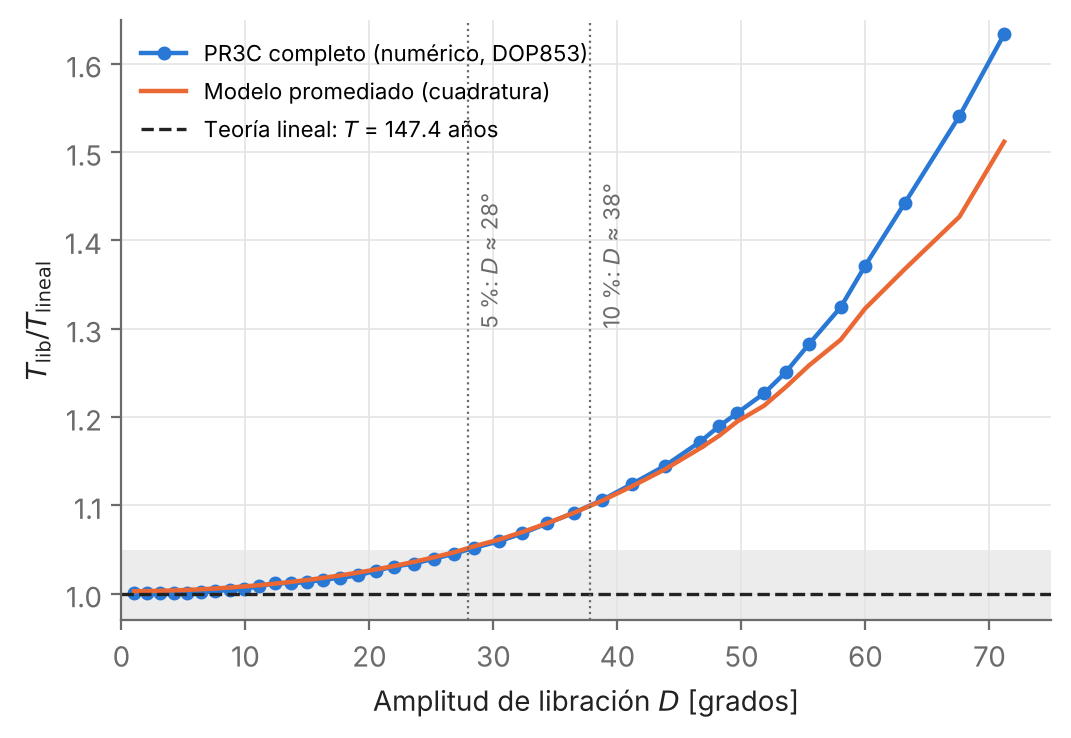
\includegraphics[width=\linewidth]{fig2_periodo_amplitud.png}\end{minipage}\hfill
\begin{minipage}{0.45\textwidth}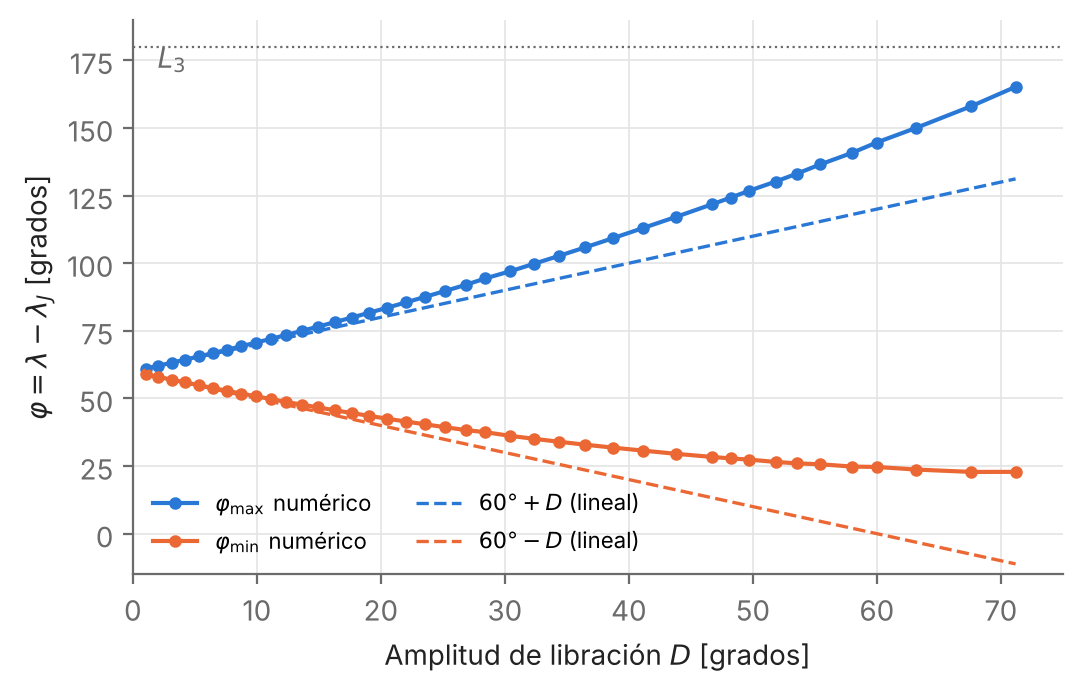
\includegraphics[width=\linewidth]{fig3_asimetria.png}\end{minipage}
\caption{\textbf{Izquierda:} período de libración relativo al lineal frente a la amplitud, en el PR3C plano (puntos), en el modelo promediado (línea naranja) y en la teoría lineal (discontinua). La banda gris marca $\pm5\,\%$. \textbf{Derecha:} puntos de retorno de $\varphi$. La teoría lineal predice una libración simétrica ($60^\circ\pm D$), pero el renacuajo real se estira hacia $L_3$ y se comprime frente a Júpiter. La forma deja de ser lineal ($\gtrsim2^\circ$ de asimetría) desde $D\approx11^\circ$, antes que el período.}
\label{fig:TD}
\end{figure}

Antes que el período falla la \emph{forma} (Fig.~\ref{fig:TD}, derecha). Júpiter repele el asteroide con más fuerza cuando este se le acerca que cuando se aleja hacia $L_3$. Por eso $\varphi_{\max}-60^\circ>60^\circ-\varphi_{\min}$ y el centro de la libración se desplaza más allá de $60^\circ$. Con $D=30^\circ$ el asteroide alcanza $\varphi_{\max}\approx97^\circ$, mientras que la teoría lineal predice $90^\circ$.

\subsection{Los troyanos reales}
La Fig.~\ref{fig:datos} (izquierda) muestra la muestra en el marco rotante: 9\,057 asteroides en $L_4$ y 5\,752 en $L_5$ (razón 1,57). Tras 2000 años de integración, la amplitud de libración tiene mediana $14{,}6^\circ$ y percentiles 5--95 de $4{,}3^\circ$--$27{,}9^\circ$ (Fig.~\ref{fig:datos}, derecha). El \textbf{95,0\,\%} de los troyanos tiene $D$ menor que el umbral del 5\,\% y el 99,9\,\% menor que el del 10\,\%. Solo 30 asteroides (0,2\,\%) escapan de la resonancia en ese tiempo, 29 de ellos en ambos modelos.

\begin{figure}[t]
\centering
\begin{minipage}{0.40\textwidth}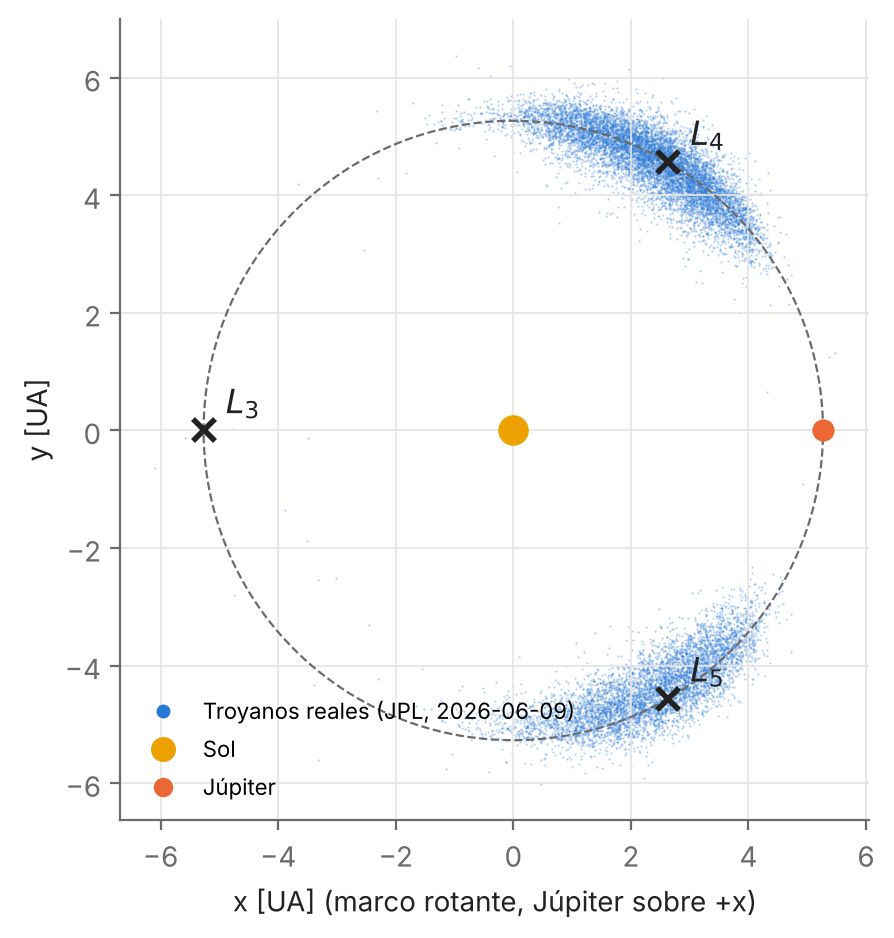
\includegraphics[width=\linewidth]{fig1_marco_rotante.png}\end{minipage}\hfill
\begin{minipage}{0.58\textwidth}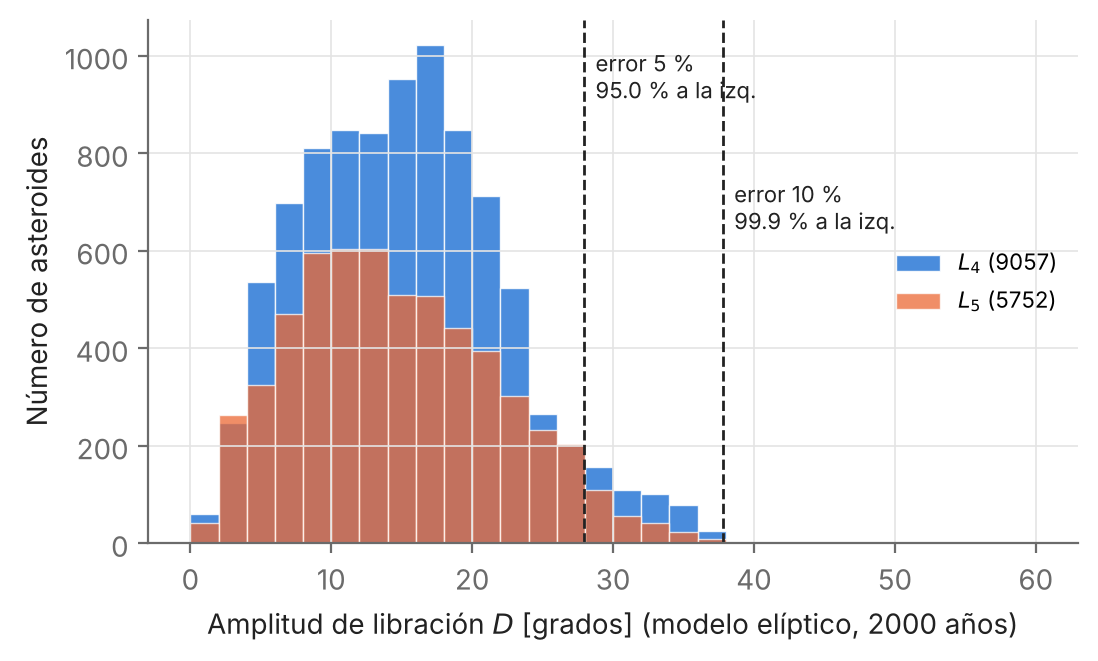
\includegraphics[width=\linewidth]{fig5_hist_amplitud.png}\end{minipage}
\caption{\textbf{Izquierda:} los 14\,809 troyanos (época 2026-06-09) en el marco que rota con Júpiter. Ocupan arcos alargados a lo largo de la órbita, no regiones pequeñas alrededor de $L_4$ y $L_5$. \textbf{Derecha:} distribución de amplitudes de libración obtenida con el modelo elíptico (histogramas superpuestos). Las líneas marcan dónde el período lineal se equivoca en un 5\,\% y en un 10\,\%. Por amplitud, casi toda la población está en el régimen \emph{cuasi}-lineal.}
\label{fig:datos}
\end{figure}

Si el único problema fuera la amplitud, el 95\,\% de los períodos estaría a menos del 5\,\% de $\Tlin$. La Fig.~\ref{fig:reales} (izquierda) muestra que no es así: solo el \textbf{67,8\,\%} lo está y apenas el 18,5\,\% está a menos del 1\,\%. Los asteroides de baja inclinación siguen la curva del PR3C plano, pero los inclinados forman bandas por encima. Para $D<10^\circ$, el período mediano es 147,5 años con $i<10^\circ$, 149,6 con $10^\circ$--$20^\circ$, 156,1 con $20^\circ$--$30^\circ$ y \textbf{162,1 años con $i>30^\circ$}. Es decir, hasta un 10\,\% más largo que el lineal, aun con amplitudes pequeñas. Físicamente, un asteroide muy inclinado pasa parte de su órbita lejos del plano de Júpiter. Allí la fuerza restauradora media es más débil y la libración, más lenta. La teoría lineal plana no contiene este efecto.

La Fig.~\ref{fig:reales} (derecha) compara dos troyanos de baja inclinación con la solución lineal de sus propias condiciones iniciales. Para $D=5^\circ$ la predicción es casi exacta. Para $D=35^\circ$ la teoría lineal subestima el máximo de $\varphi$ en casi $20^\circ$ y acumula un desfase de medio ciclo en unos 800 años. La amplitud lineal calculada a partir de $(\delta\varphi,\delta a)$ iniciales difiere de la numérica en un 8,5\,\% (mediana). Esto es razonable, porque los elementos osculantes incluyen términos de período corto.

\begin{figure}[t]
\centering
\begin{minipage}{0.50\textwidth}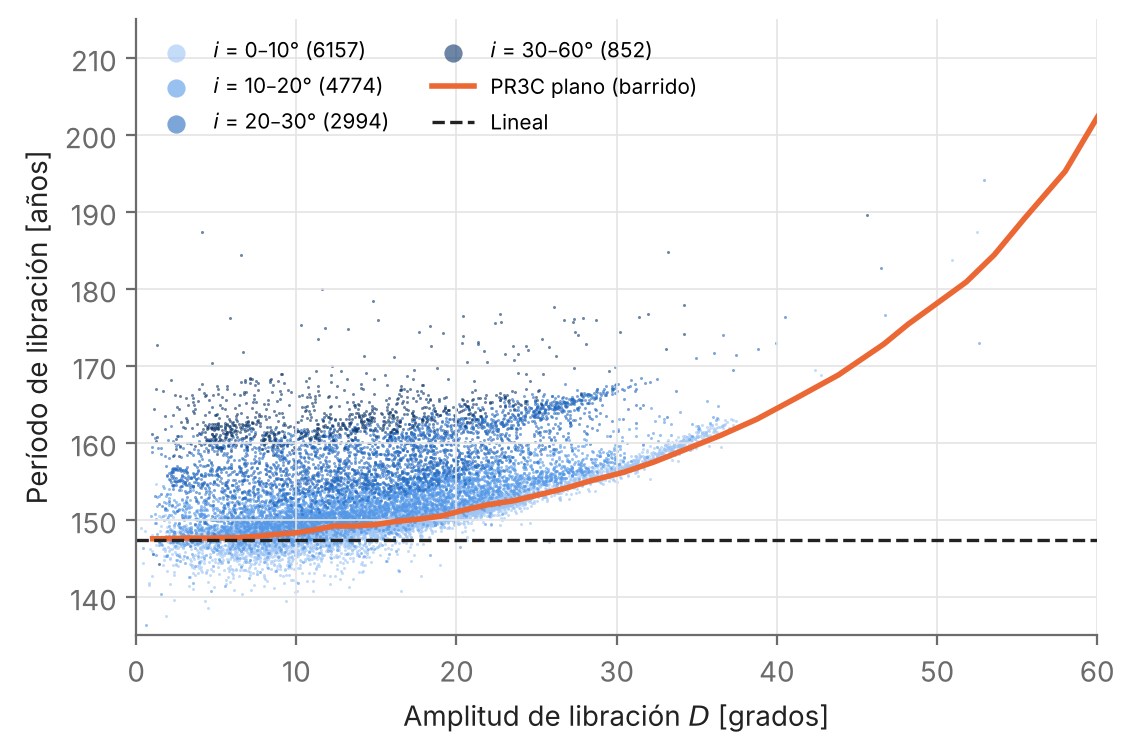
\includegraphics[width=\linewidth]{fig4_reales_T_vs_D.png}\end{minipage}\hfill
\begin{minipage}{0.48\textwidth}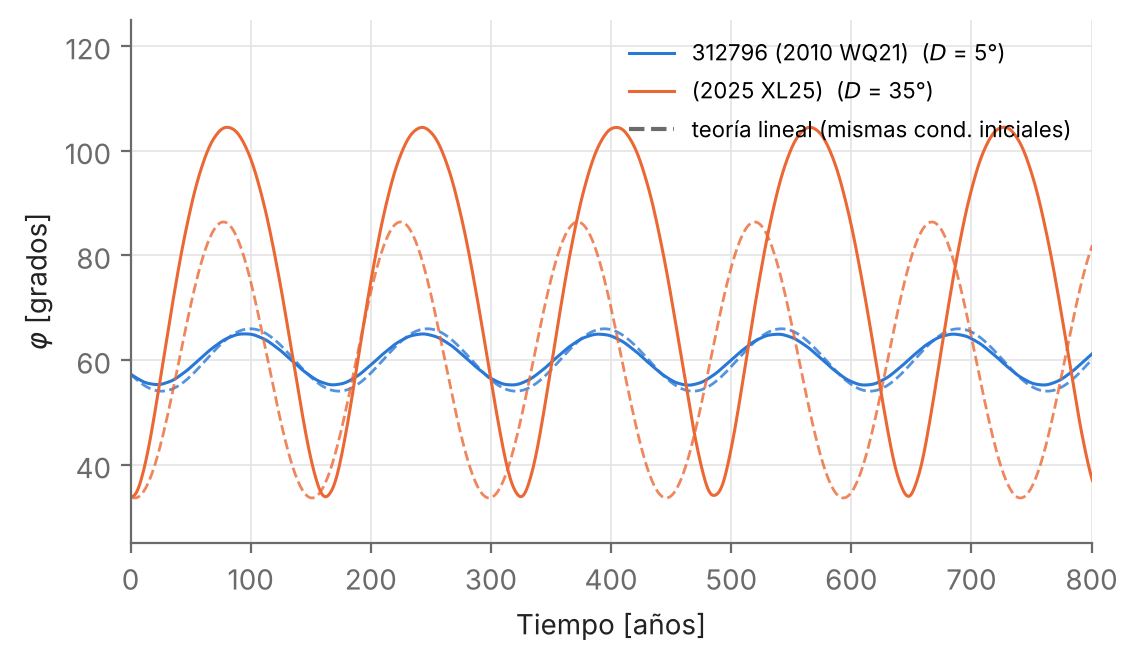
\includegraphics[width=\linewidth]{fig6_ejemplos.png}\end{minipage}
\caption{\textbf{Izquierda:} período frente a amplitud para los troyanos reales (modelo elíptico 3D), por rangos de inclinación. Los de baja inclinación siguen la curva plana (naranja). La inclinación desplaza el período hacia arriba incluso para $D$ pequeña, de modo que la amplitud no es la única fuente de error. \textbf{Derecha:} $\varphi(t)$ de dos troyanos reales (sólido) frente a la teoría lineal con las mismas condiciones iniciales (discontinua). La libración grande es asimétrica y más lenta.}
\label{fig:reales}
\end{figure}

\subsection{Una firma no lineal directamente en los datos}
El centro de los enjambres se puede medir directamente del catálogo, sin simular nada. El valor medio observado de $|\varphi|$ es $63{,}06^\circ\pm0{,}13^\circ$ en $L_4$ y $62{,}38^\circ\pm0{,}17^\circ$ en $L_5$, incompatible con los $60^\circ$ de la teoría lineal a más de $14\sigma$. El promedio temporal de nuestras integraciones da $63{,}2^\circ$ y $62{,}4^\circ$. El corrimiento es el mismo efecto de asimetría de la Fig.~\ref{fig:TD}, visto en la población real.

\subsection{Cambiar una hipótesis: circular vs.\ elíptico}
\begin{table}[h]
\centering\small
\caption{Efecto de cambiar la órbita de Júpiter de circular a elíptica, comparado con los efectos de la amplitud y de la inclinación. La excentricidad de Júpiter es la hipótesis \emph{menos} importante de las tres.}
\label{tab:comp}
\begin{tabular}{lcc}
\toprule
Cambio de hipótesis & Cambio típico en $T$ & Cambio típico en $D$\\\midrule
$e_J=0\to0{,}048$ (mismos 14\,809 asteroides) & 0,4\,\% (mediana) & $0{,}3^\circ$ (mediana), $1{,}2^\circ$ (p95)\\
$D=5^\circ\to28^\circ$ (PR3C plano) & 5\,\% & ---\\
$i<10^\circ\to i>30^\circ$ (con $D<10^\circ$) & 10\,\% & ---\\
\bottomrule
\end{tabular}
\end{table}
La Tabla~\ref{tab:comp} muestra que pasar de Júpiter circular a elíptico casi no modifica la libración: la excentricidad de Júpiter fuerza sobre todo la excentricidad del asteroide, no su ángulo resonante. Las fracciones de la Sec.~3.2 cambian menos de 2 puntos porcentuales entre los dos modelos.

\section{Conclusiones y recomendaciones}\label{sec:conc}
\begin{enumerate}\setlength\itemsep{1pt}
\item La teoría lineal alrededor de $L_4$ ($\Tlin=147{,}4$ años) se recupera exactamente en el límite $D\to0$, verificado con dos métodos independientes y con la conservación de $C_J$.
\item Su validez tiene un límite cuantificable: el período se equivoca en un 5\,\% a partir de $D\approx28^\circ$ y en un 10\,\% a partir de $D\approx38^\circ$. La asimetría del renacuajo aparece antes, desde $D\approx11^\circ$, y se observa directamente en el catálogo: los enjambres están centrados en $\approx63^\circ$, no en $60^\circ$.
\item Por amplitud, el 95\,\% de los troyanos reales está dentro del rango útil. Sin embargo, solo el 68\,\% tiene un período a menos del 5\,\% del lineal, porque la inclinación alarga la libración hasta $\sim$10\,\%. \textbf{Para la población real, el límite del análisis lineal plano lo impone la inclinación antes que la amplitud.}
\item La excentricidad de Júpiter es un efecto menor ($<1\,\%$) en escalas de $10^3$ años.
\end{enumerate}
\textbf{Respuesta a la pregunta del reto:} el análisis lineal describe cuantitativamente (error $<5\,\%$) los troyanos con $D\lesssim25^\circ$ e $i\lesssim15^\circ$. Para el resto sirve como orden de magnitud, pero no como descripción precisa.

\textbf{Recomendaciones.} (i) Extender la teoría lineal a 3D para cuantificar analíticamente el efecto de la inclinación. (ii) Incluir Saturno, cuya cercanía a la resonancia 5:2 con Júpiter controla la estabilidad de largo plazo \cite{robutel}. (iii) Comparar nuestras amplitudes con las amplitudes propias publicadas (AstDyS), que son datos independientes de nuestro ajuste.

\begin{thebibliography}{9}\small\setlength\itemsep{0pt}
\bibitem{lagrange} J.-L. Lagrange, \emph{Essai sur le problème des trois corps} (1772), Œuvres, t.~6, Gauthier-Villars.
\bibitem{szebehely} V. Szebehely, \emph{Theory of Orbits: The Restricted Problem of Three Bodies}, Academic Press (1967).
\bibitem{murray} C.~D. Murray y S.~F. Dermott, \emph{Solar System Dynamics}, Cambridge Univ.\ Press (1999), cap.~3.
\bibitem{wolf} M. Wolf, Astronomische Nachrichten \textbf{170}, 353 (1906).
\bibitem{robutel} P. Robutel y J. Bodossian, MNRAS \textbf{399}, 69--87 (2009).
\bibitem{oshima} K. Oshima y T. Yanao, Celest.\ Mech.\ Dyn.\ Astron.\ \textbf{122}, 53--74 (2015).
\bibitem{emery} J.~P. Emery et al., en \emph{Asteroids IV}, Univ.\ of Arizona Press, 203--220 (2015).
\bibitem{bottke} W.~F. Bottke et al., Space Sci.\ Rev.\ \textbf{219}, 83 (2023).
\bibitem{repo} P.~A. Ríos y J.~D. Sarmiento, repositorio del proyecto, \url{https://github.com/JuanSarmiento0719/jupiter_troyans} (2026).
\bibitem{jpl} JPL Small-Body Database y JPL Horizons, \url{https://ssd.jpl.nasa.gov} (consultados en noviembre de 2026).
\end{thebibliography}
\end{document}
